% Options for packages loaded elsewhere
\PassOptionsToPackage{unicode}{hyperref}
\PassOptionsToPackage{hyphens}{url}
%
\documentclass[
  ignorenonframetext,
]{beamer}
\usepackage{pgfpages}
\setbeamertemplate{caption}[numbered]
\setbeamertemplate{caption label separator}{: }
\setbeamercolor{caption name}{fg=normal text.fg}
\beamertemplatenavigationsymbolsempty
% Prevent slide breaks in the middle of a paragraph
\widowpenalties 1 10000
\raggedbottom
\setbeamertemplate{part page}{
  \centering
  \begin{beamercolorbox}[sep=16pt,center]{part title}
    \usebeamerfont{part title}\insertpart\par
  \end{beamercolorbox}
}
\setbeamertemplate{section page}{
  \centering
  \begin{beamercolorbox}[sep=12pt,center]{part title}
    \usebeamerfont{section title}\insertsection\par
  \end{beamercolorbox}
}
\setbeamertemplate{subsection page}{
  \centering
  \begin{beamercolorbox}[sep=8pt,center]{part title}
    \usebeamerfont{subsection title}\insertsubsection\par
  \end{beamercolorbox}
}
\AtBeginPart{
  \frame{\partpage}
}
\AtBeginSection{
  \ifbibliography
  \else
    \frame{\sectionpage}
  \fi
}
\AtBeginSubsection{
  \frame{\subsectionpage}
}
\usepackage{lmodern}
\usepackage{amssymb,amsmath}
\usepackage{ifxetex,ifluatex}
\ifnum 0\ifxetex 1\fi\ifluatex 1\fi=0 % if pdftex
  \usepackage[T1]{fontenc}
  \usepackage[utf8]{inputenc}
  \usepackage{textcomp} % provide euro and other symbols
\else % if luatex or xetex
  \usepackage{unicode-math}
  \defaultfontfeatures{Scale=MatchLowercase}
  \defaultfontfeatures[\rmfamily]{Ligatures=TeX,Scale=1}
\fi
% Use upquote if available, for straight quotes in verbatim environments
\IfFileExists{upquote.sty}{\usepackage{upquote}}{}
\IfFileExists{microtype.sty}{% use microtype if available
  \usepackage[]{microtype}
  \UseMicrotypeSet[protrusion]{basicmath} % disable protrusion for tt fonts
}{}
\makeatletter
\@ifundefined{KOMAClassName}{% if non-KOMA class
  \IfFileExists{parskip.sty}{%
    \usepackage{parskip}
  }{% else
    \setlength{\parindent}{0pt}
    \setlength{\parskip}{6pt plus 2pt minus 1pt}}
}{% if KOMA class
  \KOMAoptions{parskip=half}}
\makeatother
\usepackage{xcolor}
\IfFileExists{xurl.sty}{\usepackage{xurl}}{} % add URL line breaks if available
\IfFileExists{bookmark.sty}{\usepackage{bookmark}}{\usepackage{hyperref}}
\hypersetup{
  pdftitle={MQE: Economic Inference from Data: Module 4: Randomized Control Trials},
  pdfauthor={Claire Duquennois},
  hidelinks,
  pdfcreator={LaTeX via pandoc}}
\urlstyle{same} % disable monospaced font for URLs
\newif\ifbibliography
\usepackage{color}
\usepackage{fancyvrb}
\newcommand{\VerbBar}{|}
\newcommand{\VERB}{\Verb[commandchars=\\\{\}]}
\DefineVerbatimEnvironment{Highlighting}{Verbatim}{commandchars=\\\{\}}
% Add ',fontsize=\small' for more characters per line
\usepackage{framed}
\definecolor{shadecolor}{RGB}{248,248,248}
\newenvironment{Shaded}{\begin{snugshade}}{\end{snugshade}}
\newcommand{\AlertTok}[1]{\textcolor[rgb]{0.94,0.16,0.16}{#1}}
\newcommand{\AnnotationTok}[1]{\textcolor[rgb]{0.56,0.35,0.01}{\textbf{\textit{#1}}}}
\newcommand{\AttributeTok}[1]{\textcolor[rgb]{0.77,0.63,0.00}{#1}}
\newcommand{\BaseNTok}[1]{\textcolor[rgb]{0.00,0.00,0.81}{#1}}
\newcommand{\BuiltInTok}[1]{#1}
\newcommand{\CharTok}[1]{\textcolor[rgb]{0.31,0.60,0.02}{#1}}
\newcommand{\CommentTok}[1]{\textcolor[rgb]{0.56,0.35,0.01}{\textit{#1}}}
\newcommand{\CommentVarTok}[1]{\textcolor[rgb]{0.56,0.35,0.01}{\textbf{\textit{#1}}}}
\newcommand{\ConstantTok}[1]{\textcolor[rgb]{0.00,0.00,0.00}{#1}}
\newcommand{\ControlFlowTok}[1]{\textcolor[rgb]{0.13,0.29,0.53}{\textbf{#1}}}
\newcommand{\DataTypeTok}[1]{\textcolor[rgb]{0.13,0.29,0.53}{#1}}
\newcommand{\DecValTok}[1]{\textcolor[rgb]{0.00,0.00,0.81}{#1}}
\newcommand{\DocumentationTok}[1]{\textcolor[rgb]{0.56,0.35,0.01}{\textbf{\textit{#1}}}}
\newcommand{\ErrorTok}[1]{\textcolor[rgb]{0.64,0.00,0.00}{\textbf{#1}}}
\newcommand{\ExtensionTok}[1]{#1}
\newcommand{\FloatTok}[1]{\textcolor[rgb]{0.00,0.00,0.81}{#1}}
\newcommand{\FunctionTok}[1]{\textcolor[rgb]{0.00,0.00,0.00}{#1}}
\newcommand{\ImportTok}[1]{#1}
\newcommand{\InformationTok}[1]{\textcolor[rgb]{0.56,0.35,0.01}{\textbf{\textit{#1}}}}
\newcommand{\KeywordTok}[1]{\textcolor[rgb]{0.13,0.29,0.53}{\textbf{#1}}}
\newcommand{\NormalTok}[1]{#1}
\newcommand{\OperatorTok}[1]{\textcolor[rgb]{0.81,0.36,0.00}{\textbf{#1}}}
\newcommand{\OtherTok}[1]{\textcolor[rgb]{0.56,0.35,0.01}{#1}}
\newcommand{\PreprocessorTok}[1]{\textcolor[rgb]{0.56,0.35,0.01}{\textit{#1}}}
\newcommand{\RegionMarkerTok}[1]{#1}
\newcommand{\SpecialCharTok}[1]{\textcolor[rgb]{0.00,0.00,0.00}{#1}}
\newcommand{\SpecialStringTok}[1]{\textcolor[rgb]{0.31,0.60,0.02}{#1}}
\newcommand{\StringTok}[1]{\textcolor[rgb]{0.31,0.60,0.02}{#1}}
\newcommand{\VariableTok}[1]{\textcolor[rgb]{0.00,0.00,0.00}{#1}}
\newcommand{\VerbatimStringTok}[1]{\textcolor[rgb]{0.31,0.60,0.02}{#1}}
\newcommand{\WarningTok}[1]{\textcolor[rgb]{0.56,0.35,0.01}{\textbf{\textit{#1}}}}
\usepackage{longtable,booktabs}
\usepackage{caption}
% Make caption package work with longtable
\makeatletter
\def\fnum@table{\tablename~\thetable}
\makeatother
\usepackage{graphicx}
\makeatletter
\def\maxwidth{\ifdim\Gin@nat@width>\linewidth\linewidth\else\Gin@nat@width\fi}
\def\maxheight{\ifdim\Gin@nat@height>\textheight\textheight\else\Gin@nat@height\fi}
\makeatother
% Scale images if necessary, so that they will not overflow the page
% margins by default, and it is still possible to overwrite the defaults
% using explicit options in \includegraphics[width, height, ...]{}
\setkeys{Gin}{width=\maxwidth,height=\maxheight,keepaspectratio}
% Set default figure placement to htbp
\makeatletter
\def\fps@figure{htbp}
\makeatother
\setlength{\emergencystretch}{3em} % prevent overfull lines
\providecommand{\tightlist}{%
  \setlength{\itemsep}{0pt}\setlength{\parskip}{0pt}}
\setcounter{secnumdepth}{-\maxdimen} % remove section numbering

\title{MQE: Economic Inference from Data:\\
Module 4: Randomized Control Trials}
\author{Claire Duquennois}
\date{6/9/2020}

\begin{document}
\frame{\titlepage}

\begin{frame}{The Experimental Ideal:}
\protect\hypertarget{the-experimental-ideal}{}
Getting causal effects is HARD!
\end{frame}

\begin{frame}{The Experimental Ideal:}
\protect\hypertarget{the-experimental-ideal-1}{}
Getting causal effects is HARD!

So where do we go from here?

Randomized control trials (RCT's) aka the ``Gold standard'' of
experimental designs
\end{frame}

\begin{frame}{Random assignment and the selection problem}
\protect\hypertarget{random-assignment-and-the-selection-problem}{}
The idea: use random assignment to remove selection bias

Suppose a constant treatment effect: \(Y_i(1)-Y_i(0)=\tau\). For
observation \(i\) we have that

\[
\begin{split}
Y_i &=Y_i(0)+\tau D_i\\
Y_i &=E[Y_i(0)]+\tau D_i+Y_i(0)-E[Y_i(0)]\\
Y_i &=\alpha+\tau D_i+\eta_i
\end{split}
\]

where \(\alpha=E[Y_i(0)]\), \(\tau=Y_i(1)-Y_i(0)\), and \(\eta_i\) is
the random part of \(Y_i(0)\) since \(\eta_i=Y_i(0)-E[Y_i(0)]\).
\end{frame}

\begin{frame}{Random assignment and the selection problem}
\protect\hypertarget{random-assignment-and-the-selection-problem-1}{}
The expected outcomes for someone with treatment \((D_i=1)\), and
without treatment \((D_i=0)\) are given by

\[
\begin{split}
E[Y_i(1)] &=\alpha +\tau +E[\eta_i|D_i=1]\\
E[Y_i(0)] &=\alpha +E[\eta_i|D_i=0]\\
\end{split}
\] so that we can break down the difference between these outcomes as \[
E[Y_i(1)]-E[Y_i(0)] = 
    \underbrace{\tau}_\text{treatment effect} + \underbrace{E[\eta_i|D_i=1]-E[\eta_i|D_i=0]}_\text{selection bias}.
\]
\end{frame}

\begin{frame}{Random assignment and the selection problem}
\protect\hypertarget{random-assignment-and-the-selection-problem-2}{}
Selection bias will bias our estimate of \(\tau\) if those who select
into treatment have a different expected outcome compared to those who
do not select into treatment: \[
E[Y_i(0)|D_i=1]\neq E[Y_i(0)|D_i=0].
\]

This is because treatment is not random:
\(\{Y_i(1), Y_i(0)\}\not\perp D_i\).
\end{frame}

\begin{frame}{Random assignment and the selection problem}
\protect\hypertarget{random-assignment-and-the-selection-problem-3}{}
There is no reason to believe that those who select into treatment have
the same expected outcome as those who do not, if they were to be
treated, that is to say, it is possible (and even likely) that

\[
\underbrace{E[Y_i(0)|D_i=0]}_\text{observed}\neq  \underbrace{E[Y_i(0)|D_i=1]}_\text{unobserved}\neq E[Y_i(0)]
\]
\end{frame}

\begin{frame}{Random assignment and the selection problem}
\protect\hypertarget{random-assignment-and-the-selection-problem-4}{}
The conditional independence assumption allows us to control for
selection bias by conditioning on \textbf{observed
characteristics}\ldots{}

\ldots{} \textbf{unobserved characteristics} that we cannot control for
will often also bias our estimates.

Random assignment solves all of these selection bias problems.
\end{frame}

\begin{frame}{Random assignment and the selection problem}
\protect\hypertarget{random-assignment-and-the-selection-problem-5}{}
Random assignment makes \(D_i\) independent of potential outcomes:

\[
\{Y_i(1), Y_i(0)\}\perp  D_i.
\]

With random assignment, we know that in expectation,

\[
\underbrace{E[Y_i(0)|D_i=0]}_\text{observed}=  \underbrace{E[Y_i(0)|D_i=1]}_\text{unobserved}= E[Y_i(0)]
\]

\begin{center}
and
\end{center}

\[
\underbrace{E[Y_i(1)|D_i=0]}_\text{unobserved}= \underbrace{E[Y_i(1)|D_i=1]}_\text{observed}= E[Y_i(1)]
\]
\end{frame}

\begin{frame}{Random assignment and the selection problem}
\protect\hypertarget{random-assignment-and-the-selection-problem-6}{}
Thus, the causal \textbf{Average Treatment Effect (ATE)},
\(\bar{\tau}\), is\\
\footnotesize \[
\begin{aligned}
\bar{\tau}&=E[Y_i(1)]-E[Y_i(0)]=\underbrace{E[Y_i(1)|D_i=1]}_\text{observed}-\underbrace{E[Y_i(0)|D_i=0]}_\text{observed}\\
&=E[Y_i|D_i=1]-E[Y_i|D_i=0].
\end{aligned}
\] \normalsize

and we can easily estimate \(\bar{\tau}\), by taking the difference
between the average value of \(Y_i\) in the treatment group and the
average value of \(Y_i\) in the control group.
\end{frame}

\begin{frame}{RCT estimation}
\protect\hypertarget{rct-estimation}{}
RCT regressions are about as straightforward as it gets.

As modeled above, you can estimate

\[
Y_i=\alpha+\tau D_i+\eta_i
\]

where \(\alpha=E[Y_i(0)]\), \(\tau=Y_i(1)-Y_i(0)\), and \(\eta_i\) is
the random error term.
\end{frame}

\begin{frame}{RCT estimation}
\protect\hypertarget{rct-estimation-1}{}
The treatment effect will be given by \[
E[Y_i(1)]-E[Y_i(0)] = 
    \underbrace{\tau}_\text{treatment effect} + \underbrace{E[\eta_i|D_i=1]-E[\eta_i|D_i=0]}_\text{selection bias}.
\] With proper randomization,

\[
E[\eta_i|D_i=1]= E[\eta_i|D_i=0]
\] so there is no selection bias giving us an unbiased estimate of
\(\tau\).
\end{frame}

\begin{frame}{RCT Simulation}
\protect\hypertarget{rct-simulation}{}
I am a principal of a large school and I want to evaluate how access to
small reading groups with a paraprofessional helps improve 4th grade
test scores.

I take all the 4th graders and randomly assign 30 percent of them to
treatment (participating in the reading groups). The control group
continued class as normal.
\end{frame}

\begin{frame}[fragile]{RCT Simulation}
\protect\hypertarget{rct-simulation-1}{}
I generate a set of simulated data: \tiny

\begin{Shaded}
\begin{Highlighting}[]
\KeywordTok{set.seed}\NormalTok{(}\DecValTok{1999}\NormalTok{)}

\NormalTok{scores5\textless{}{-}}\KeywordTok{as.data.frame}\NormalTok{(}\KeywordTok{rep}\NormalTok{(}\KeywordTok{c}\NormalTok{(}\DecValTok{1}\NormalTok{,}\DecValTok{2}\NormalTok{,}\DecValTok{3}\NormalTok{,}\DecValTok{4}\NormalTok{,}\DecValTok{5}\NormalTok{,}\DecValTok{6}\NormalTok{,}\DecValTok{7}\NormalTok{,}\DecValTok{8}\NormalTok{,}\DecValTok{9}\NormalTok{,}\DecValTok{10}\NormalTok{),}\DataTypeTok{times=}\DecValTok{30}\NormalTok{))}
\KeywordTok{names}\NormalTok{(scores5)\textless{}{-}}\KeywordTok{c}\NormalTok{(}\StringTok{"class"}\NormalTok{)}
\NormalTok{scores5 \textless{}{-}}\StringTok{ }\NormalTok{fastDummies}\OperatorTok{::}\KeywordTok{dummy\_cols}\NormalTok{(scores5, }\DataTypeTok{select\_columns =} \StringTok{"class"}\NormalTok{)}
\NormalTok{scores5}\OperatorTok{$}\NormalTok{error\textless{}{-}}\KeywordTok{rnorm}\NormalTok{(}\DecValTok{300}\NormalTok{, }\DataTypeTok{mean=}\DecValTok{0}\NormalTok{, }\DataTypeTok{sd=}\DecValTok{10}\NormalTok{)}

\CommentTok{\#treatment indicator}
\NormalTok{scores5}\OperatorTok{$}\NormalTok{treat\textless{}{-}}\KeywordTok{rbinom}\NormalTok{(}\DecValTok{300}\NormalTok{,}\DecValTok{1}\NormalTok{,}\FloatTok{0.3}\NormalTok{)}

\CommentTok{\#mean reading score}
\NormalTok{alpha=}\DecValTok{75}

\CommentTok{\#treatment effect}
\NormalTok{tau=}\DecValTok{10}

\CommentTok{\#the data generating process: notice the class does affect a student\textquotesingle{}s score}
\NormalTok{scores5}\OperatorTok{$}\NormalTok{read4\textless{}{-}(alpha}\OperatorTok{+}\NormalTok{tau}\OperatorTok{*}\NormalTok{scores5}\OperatorTok{$}\NormalTok{treat}\OperatorTok{+}\NormalTok{scores5}\OperatorTok{$}\NormalTok{error}
                \OperatorTok{+}\DecValTok{4}\OperatorTok{*}\NormalTok{scores5}\OperatorTok{$}\NormalTok{class\_}\DecValTok{1}\OperatorTok{+}\NormalTok{(}\OperatorTok{{-}}\DecValTok{6}\NormalTok{)}\OperatorTok{*}\NormalTok{scores5}\OperatorTok{$}\NormalTok{class\_}\DecValTok{2}\OperatorTok{+}\DecValTok{8}\OperatorTok{*}\NormalTok{scores5}\OperatorTok{$}\NormalTok{class\_}\DecValTok{3}
                \OperatorTok{+}\NormalTok{(}\OperatorTok{{-}}\DecValTok{4}\NormalTok{)}\OperatorTok{*}\NormalTok{scores5}\OperatorTok{$}\NormalTok{class\_}\DecValTok{4}\OperatorTok{+}\DecValTok{7}\OperatorTok{*}\NormalTok{scores5}\OperatorTok{$}\NormalTok{class\_}\DecValTok{5}\OperatorTok{+}\NormalTok{(}\OperatorTok{{-}}\DecValTok{2}\NormalTok{)}\OperatorTok{*}\NormalTok{scores5}\OperatorTok{$}\NormalTok{class\_}\DecValTok{6}
                \OperatorTok{+}\DecValTok{5}\OperatorTok{*}\NormalTok{scores5}\OperatorTok{$}\NormalTok{class\_}\DecValTok{7}\OperatorTok{+}\NormalTok{(}\OperatorTok{{-}}\DecValTok{10}\NormalTok{)}\OperatorTok{*}\NormalTok{scores5}\OperatorTok{$}\NormalTok{class\_}\DecValTok{8}
                \OperatorTok{+}\DecValTok{8}\OperatorTok{*}\NormalTok{scores5}\OperatorTok{$}\NormalTok{class\_}\DecValTok{9}\OperatorTok{+}\DecValTok{4}\OperatorTok{*}\NormalTok{scores5}\OperatorTok{$}\NormalTok{class\_}\DecValTok{10}\NormalTok{)}
\end{Highlighting}
\end{Shaded}
\end{frame}

\begin{frame}[fragile]{RCT Simulation}
\protect\hypertarget{rct-simulation-2}{}
\tiny

\begin{Shaded}
\begin{Highlighting}[]
\NormalTok{rct1\textless{}{-}}\KeywordTok{felm}\NormalTok{(read4}\OperatorTok{\textasciitilde{}}\NormalTok{treat,scores5)}
\KeywordTok{stargazer}\NormalTok{(rct1, }\DataTypeTok{type=}\StringTok{"latex"}\NormalTok{, }\DataTypeTok{header=}\OtherTok{FALSE}\NormalTok{)}
\end{Highlighting}
\end{Shaded}

\begin{table}[!htbp] \centering 
  \caption{} 
  \label{} 
\begin{tabular}{@{\extracolsep{5pt}}lc} 
\\[-1.8ex]\hline 
\hline \\[-1.8ex] 
 & \multicolumn{1}{c}{\textit{Dependent variable:}} \\ 
\cline{2-2} 
\\[-1.8ex] & read4 \\ 
\hline \\[-1.8ex] 
 treat & 11.229$^{***}$ \\ 
  & (1.442) \\ 
  & \\ 
 Constant & 77.150$^{***}$ \\ 
  & (0.750) \\ 
  & \\ 
\hline \\[-1.8ex] 
Observations & 300 \\ 
R$^{2}$ & 0.169 \\ 
Adjusted R$^{2}$ & 0.166 \\ 
Residual Std. Error & 11.092 (df = 298) \\ 
\hline 
\hline \\[-1.8ex] 
\textit{Note:}  & \multicolumn{1}{r}{$^{*}$p$<$0.1; $^{**}$p$<$0.05; $^{***}$p$<$0.01} \\ 
\end{tabular} 
\end{table}

\normalsize

Because treatment was randomized, even though the class the student is
in does affect their score, we recover an unbiased estimate of the true
treatment effect (\(\tau=10\)).
\end{frame}

\begin{frame}{RCT Key assumption}
\protect\hypertarget{rct-key-assumption}{}
The key assumption is that \[
E[\eta_i|D_i=1]= E[\eta_i|D_i=0]=0.
\]

\begin{itemize}
\item
  we cannot test this assumption directly
\item
  BUT we can do a \textbf{balance test}: we check to see if observable
  characteristics among treatment and control groups are the same on
  average.
\end{itemize}
\end{frame}

\begin{frame}{RCT Balance tests}
\protect\hypertarget{rct-balance-tests}{}
\begin{itemize}
\item
  can be presented as a table of the following regressions
  \(X_i=\beta_0+\beta_1D_i+\epsilon_i\) where \(X_i\) is a vector of
  characteristics being tested.
\item
  are often presented as simple t-test tables testing the difference in
  means between the treatment and control groups.
\end{itemize}
\end{frame}

\begin{frame}{RCT Balance Tests}
\protect\hypertarget{rct-balance-tests-1}{}
Balance test variables should be

\begin{itemize}
\item
  characteristics at baseline, prior to treatment,
\item
  or characteristics that would be unaffected by treatment.
\end{itemize}

\textbf{Why?}

Select good variables to include in our balance test.

\(\Rightarrow\) TopHat
\end{frame}

\begin{frame}{RCT Balance Tests}
\protect\hypertarget{rct-balance-tests-2}{}
Balance tests are often run on many variables:

\begin{itemize}
\item
  some may come up with a statistically significant difference by simple
  random chance
\item
  if many are significantly different, this is a red flag that the key
  assumption does not hold
\item
  If an unbalanced variable is of particular concern you may want to
  control for it and/or keep it in mind in your interpretation of
  results
\end{itemize}
\end{frame}

\begin{frame}{RCT Simulation}
\protect\hypertarget{rct-simulation-3}{}
Suppose the principal is concerned that there were some problems with
the randomization.

She has access to some additional data. She adds it to her data set and
does a balance test.
\end{frame}

\begin{frame}[fragile]{RCT Simulation}
\protect\hypertarget{rct-simulation-4}{}
\tiny

\begin{Shaded}
\begin{Highlighting}[]
\CommentTok{\#simulating covariates}

\CommentTok{\#third grade test scores. Notice I am generateing simulated academic scores }
\CommentTok{\#that have a correlation to their "untreated" performance in 4th grade reading}
\NormalTok{scores5}\OperatorTok{$}\NormalTok{read3\textless{}{-}alpha}\OperatorTok{+}\NormalTok{scores5}\OperatorTok{$}\NormalTok{error}\OperatorTok{+}\KeywordTok{rnorm}\NormalTok{(}\DecValTok{300}\NormalTok{,}\DecValTok{3}\NormalTok{,}\DecValTok{2}\NormalTok{)}
\NormalTok{scores5}\OperatorTok{$}\NormalTok{math3\textless{}{-}alpha}\OperatorTok{+}\NormalTok{scores5}\OperatorTok{$}\NormalTok{error}\OperatorTok{+}\KeywordTok{rnorm}\NormalTok{(}\DecValTok{300}\NormalTok{,}\DecValTok{15}\NormalTok{,}\DecValTok{2}\NormalTok{)}
\NormalTok{scores5}\OperatorTok{$}\NormalTok{hist3\textless{}{-}alpha}\OperatorTok{+}\NormalTok{scores5}\OperatorTok{$}\NormalTok{error}\OperatorTok{+}\KeywordTok{rnorm}\NormalTok{(}\DecValTok{300}\NormalTok{,}\DecValTok{5}\NormalTok{,}\DecValTok{2}\NormalTok{)}
\NormalTok{scores5}\OperatorTok{$}\NormalTok{pe3\textless{}{-}}\KeywordTok{rnorm}\NormalTok{(}\DecValTok{300}\NormalTok{,}\DecValTok{90}\NormalTok{,}\DecValTok{2}\NormalTok{)}

\CommentTok{\#other 4th grade test scores: notice I am generating scores that correlated }
\CommentTok{\#with their subject performance in 3rd grade. Also, the treatment is }
\CommentTok{\#affecting other 4th grade academic scores}
\NormalTok{scores5}\OperatorTok{$}\NormalTok{hist4\textless{}{-}}\DecValTok{4}\OperatorTok{*}\NormalTok{scores5}\OperatorTok{$}\NormalTok{treat}\OperatorTok{+}\NormalTok{scores5}\OperatorTok{$}\NormalTok{hist3}\OperatorTok{+}\KeywordTok{rnorm}\NormalTok{(}\DecValTok{300}\NormalTok{,}\OperatorTok{{-}}\DecValTok{2}\NormalTok{,}\DecValTok{2}\NormalTok{)}
\NormalTok{scores5}\OperatorTok{$}\NormalTok{pe4\textless{}{-}scores5}\OperatorTok{$}\NormalTok{pe3}\OperatorTok{+}\KeywordTok{rnorm}\NormalTok{(}\DecValTok{300}\NormalTok{,}\DecValTok{0}\NormalTok{,}\DecValTok{5}\NormalTok{)}
\NormalTok{scores5}\OperatorTok{$}\NormalTok{math4\textless{}{-}}\DecValTok{2}\OperatorTok{*}\NormalTok{scores5}\OperatorTok{$}\NormalTok{treat}\OperatorTok{+}\NormalTok{scores5}\OperatorTok{$}\NormalTok{math3}\OperatorTok{+}\KeywordTok{rnorm}\NormalTok{(}\DecValTok{300}\NormalTok{,}\OperatorTok{{-}}\DecValTok{5}\NormalTok{,}\DecValTok{3}\NormalTok{)}

\CommentTok{\#student characteristics}
\NormalTok{scores5}\OperatorTok{$}\NormalTok{female\textless{}{-}}\KeywordTok{rbinom}\NormalTok{(}\DecValTok{300}\NormalTok{,}\DecValTok{1}\NormalTok{,}\FloatTok{0.5}\NormalTok{)}
\NormalTok{scores5}\OperatorTok{$}\NormalTok{age\textless{}{-}}\KeywordTok{runif}\NormalTok{(}\DecValTok{300}\NormalTok{,}\DecValTok{9}\NormalTok{,}\DecValTok{10}\NormalTok{)}
\NormalTok{scores5}\OperatorTok{$}\NormalTok{height\textless{}{-}}\KeywordTok{rnorm}\NormalTok{(}\DecValTok{300}\NormalTok{,}\FloatTok{1.3}\NormalTok{,}\FloatTok{0.2}\NormalTok{)}

\NormalTok{scoresmini\textless{}{-}scores5[,}\KeywordTok{c}\NormalTok{(}\StringTok{"treat"}\NormalTok{, }\StringTok{"read4"}\NormalTok{, }\StringTok{"read3"}\NormalTok{, }\StringTok{"math3"}\NormalTok{,}\StringTok{"hist3"}\NormalTok{,}\StringTok{"pe3"}\NormalTok{,}\StringTok{"hist4"}\NormalTok{,}\StringTok{"pe4"}\NormalTok{,}\StringTok{"math4"}\NormalTok{,}\StringTok{"female"}\NormalTok{, }\StringTok{"age"}\NormalTok{, }\StringTok{"height"}\NormalTok{)]}
\NormalTok{knitr}\OperatorTok{::}\KeywordTok{kable}\NormalTok{(}\KeywordTok{head}\NormalTok{(scoresmini))}
\end{Highlighting}
\end{Shaded}

\begin{longtable}[]{@{}rrrrrrrrrrrr@{}}
\toprule
treat & read4 & read3 & math3 & hist3 & pe3 & hist4 & pe4 & math4 &
female & age & height\tabularnewline
\midrule
\endhead
0 & 86.32672 & 83.27039 & 96.31086 & 87.68543 & 91.03541 & 88.16632 &
93.95379 & 94.98303 & 0 & 9.597192 & 1.455253\tabularnewline
0 & 68.62170 & 79.22211 & 88.71313 & 79.91069 & 93.06738 & 76.14878 &
94.28598 & 81.82348 & 1 & 9.262324 & 1.463210\tabularnewline
1 & 105.03009 & 87.89982 & 102.82710 & 92.07489 & 86.74861 & 95.05262 &
82.04735 & 102.39419 & 1 & 9.029675 & 1.720607\tabularnewline
0 & 85.69802 & 94.08272 & 101.67523 & 95.73204 & 88.38979 & 94.73489 &
76.42173 & 97.08292 & 1 & 9.896365 & 1.319147\tabularnewline
0 & 83.33690 & 74.47617 & 90.96568 & 80.65065 & 93.68531 & 77.05651 &
86.33431 & 84.26472 & 1 & 9.792383 & 1.088095\tabularnewline
0 & 78.19827 & 80.55488 & 96.59311 & 84.92801 & 87.12997 & 83.51559 &
93.56600 & 92.40844 & 1 & 9.635341 & 1.124679\tabularnewline
\bottomrule
\end{longtable}
\end{frame}

\begin{frame}[fragile]{RCT Simulation}
\protect\hypertarget{rct-simulation-5}{}
\tiny

\begin{Shaded}
\begin{Highlighting}[]
\CommentTok{\#as you can see, we have simulated some complex interrelationships between theses variables.}
\KeywordTok{cor}\NormalTok{(scoresmini)}
\end{Highlighting}
\end{Shaded}

\begin{verbatim}
##               treat        read4       read3        math3        hist3
## treat   1.000000000  0.411103370  0.06210422  0.043810660  0.048985855
## read4   0.411103370  1.000000000  0.76370646  0.756595945  0.767164090
## read3   0.062104220  0.763706465  1.00000000  0.954947392  0.957691240
## math3   0.043810660  0.756595945  0.95494739  1.000000000  0.951163232
## hist3   0.048985855  0.767164090  0.95769124  0.951163232  1.000000000
## pe3    -0.134794987 -0.078928737  0.01977274  0.025802541  0.002345894
## hist4   0.210104738  0.799439890  0.92717436  0.910566252  0.965319194
## pe4    -0.043975444  0.001522679  0.06059868  0.067988360  0.044767865
## math4   0.140564617  0.764954614  0.92332515  0.951489208  0.917393931
## female  0.003009974 -0.019753464  0.01298834  0.002850811 -0.014423484
## age     0.069344630 -0.046119854 -0.09536580 -0.096909858 -0.103607528
## height -0.049395136  0.055676186  0.04243414  0.032683477  0.040917764
##                 pe3       hist4          pe4       math4       female
## treat  -0.134794987  0.21010474 -0.043975444  0.14056462  0.003009974
## read4  -0.078928737  0.79943989  0.001522679  0.76495461 -0.019753464
## read3   0.019772739  0.92717436  0.060598681  0.92332515  0.012988341
## math3   0.025802541  0.91056625  0.067988360  0.95148921  0.002850811
## hist3   0.002345894  0.96531919  0.044767865  0.91739393 -0.014423484
## pe3     1.000000000 -0.02968731  0.472814327  0.02354280  0.026070397
## hist4  -0.029687311  1.00000000  0.017628038  0.89351172 -0.017902077
## pe4     0.472814327  0.01762804  1.000000000  0.05519176 -0.013560064
## math4   0.023542799  0.89351172  0.055191759  1.00000000  0.034182940
## female  0.026070397 -0.01790208 -0.013560064  0.03418294  1.000000000
## age    -0.045765250 -0.08045850 -0.036665854 -0.11731677 -0.070468503
## height  0.046935386  0.03323997 -0.019725022  0.01223729 -0.079529570
##                age      height
## treat   0.06934463 -0.04939514
## read4  -0.04611985  0.05567619
## read3  -0.09536580  0.04243414
## math3  -0.09690986  0.03268348
## hist3  -0.10360753  0.04091776
## pe3    -0.04576525  0.04693539
## hist4  -0.08045850  0.03323997
## pe4    -0.03666585 -0.01972502
## math4  -0.11731677  0.01223729
## female -0.07046850 -0.07952957
## age     1.00000000  0.01430370
## height  0.01430370  1.00000000
\end{verbatim}
\end{frame}

\begin{frame}[fragile]{RCT Simulation}
\protect\hypertarget{rct-simulation-6}{}
\tiny

\begin{Shaded}
\begin{Highlighting}[]
\NormalTok{namevec\textless{}{-}}\KeywordTok{names}\NormalTok{(scores5)}
\CommentTok{\#selecting variables to test}
\NormalTok{namevec\textless{}{-}namevec[}\OperatorTok{!}\NormalTok{namevec}\OperatorTok{\%in\%}\KeywordTok{c}\NormalTok{(}\StringTok{"class"}\NormalTok{,}\StringTok{"error"}\NormalTok{, }\StringTok{"treat"}\NormalTok{,}\StringTok{"read4"}\NormalTok{)]}

\CommentTok{\#generating the syntax that will go in the lm function with a loop}
\NormalTok{allModelsList \textless{}{-}}\StringTok{ }\KeywordTok{lapply}\NormalTok{(}\KeywordTok{paste}\NormalTok{(namevec,}\StringTok{"\textasciitilde{}treat"}\NormalTok{), as.formula)}

\CommentTok{\#running all of the balance tests with a loop}
\NormalTok{allModelsResults \textless{}{-}}\StringTok{ }\KeywordTok{lapply}\NormalTok{(allModelsList, }\ControlFlowTok{function}\NormalTok{(x) }\KeywordTok{lm}\NormalTok{(x, scores5))  }
\end{Highlighting}
\end{Shaded}
\end{frame}

\begin{frame}[fragile]{RCT Simulation}
\protect\hypertarget{rct-simulation-7}{}
\tiny

\begin{Shaded}
\begin{Highlighting}[]
\KeywordTok{stargazer}\NormalTok{(allModelsResults[[}\DecValTok{1}\NormalTok{]],allModelsResults[[}\DecValTok{2}\NormalTok{]],allModelsResults[[}\DecValTok{3}\NormalTok{]],}
\NormalTok{          allModelsResults[[}\DecValTok{4}\NormalTok{]], allModelsResults[[}\DecValTok{5}\NormalTok{]], }\DataTypeTok{type=}\StringTok{"latex"}\NormalTok{, }\DataTypeTok{header=}\OtherTok{FALSE}\NormalTok{)}
\end{Highlighting}
\end{Shaded}

\begin{table}[!htbp] \centering 
  \caption{} 
  \label{} 
\begin{tabular}{@{\extracolsep{5pt}}lccccc} 
\\[-1.8ex]\hline 
\hline \\[-1.8ex] 
 & \multicolumn{5}{c}{\textit{Dependent variable:}} \\ 
\cline{2-6} 
\\[-1.8ex] & class\_1 & class\_2 & class\_3 & class\_4 & class\_5 \\ 
\\[-1.8ex] & (1) & (2) & (3) & (4) & (5)\\ 
\hline \\[-1.8ex] 
 treat & $-$0.019 & 0.049 & $-$0.052 & $-$0.052 & $-$0.036 \\ 
  & (0.039) & (0.039) & (0.039) & (0.039) & (0.039) \\ 
  & & & & & \\ 
 Constant & 0.105$^{***}$ & 0.087$^{***}$ & 0.114$^{***}$ & 0.114$^{***}$ & 0.110$^{***}$ \\ 
  & (0.020) & (0.020) & (0.020) & (0.020) & (0.020) \\ 
  & & & & & \\ 
\hline \\[-1.8ex] 
Observations & 300 & 300 & 300 & 300 & 300 \\ 
R$^{2}$ & 0.001 & 0.005 & 0.006 & 0.006 & 0.003 \\ 
Adjusted R$^{2}$ & $-$0.003 & 0.002 & 0.003 & 0.003 & $-$0.001 \\ 
Residual Std. Error (df = 298) & 0.301 & 0.300 & 0.300 & 0.300 & 0.301 \\ 
F Statistic (df = 1; 298) & 0.226 & 1.578 & 1.805 & 1.805 & 0.825 \\ 
\hline 
\hline \\[-1.8ex] 
\textit{Note:}  & \multicolumn{5}{r}{$^{*}$p$<$0.1; $^{**}$p$<$0.05; $^{***}$p$<$0.01} \\ 
\end{tabular} 
\end{table}
\end{frame}

\begin{frame}[fragile]{RCT Simulation}
\protect\hypertarget{rct-simulation-8}{}
\tiny

\begin{Shaded}
\begin{Highlighting}[]
\KeywordTok{stargazer}\NormalTok{(allModelsResults[[}\DecValTok{6}\NormalTok{]],allModelsResults[[}\DecValTok{7}\NormalTok{]],allModelsResults[[}\DecValTok{8}\NormalTok{]],}
\NormalTok{          allModelsResults[[}\DecValTok{9}\NormalTok{]], allModelsResults[[}\DecValTok{10}\NormalTok{]], }\DataTypeTok{type=}\StringTok{"latex"}\NormalTok{, }\DataTypeTok{header=}\OtherTok{FALSE}\NormalTok{)}
\end{Highlighting}
\end{Shaded}

\begin{table}[!htbp] \centering 
  \caption{} 
  \label{} 
\begin{tabular}{@{\extracolsep{5pt}}lccccc} 
\\[-1.8ex]\hline 
\hline \\[-1.8ex] 
 & \multicolumn{5}{c}{\textit{Dependent variable:}} \\ 
\cline{2-6} 
\\[-1.8ex] & class\_6 & class\_7 & class\_8 & class\_9 & class\_10 \\ 
\\[-1.8ex] & (1) & (2) & (3) & (4) & (5)\\ 
\hline \\[-1.8ex] 
 treat & 0.066$^{*}$ & 0.015 & $-$0.052 & 0.015 & 0.066$^{*}$ \\ 
  & (0.039) & (0.039) & (0.039) & (0.039) & (0.039) \\ 
  & & & & & \\ 
 Constant & 0.082$^{***}$ & 0.096$^{***}$ & 0.114$^{***}$ & 0.096$^{***}$ & 0.082$^{***}$ \\ 
  & (0.020) & (0.020) & (0.020) & (0.020) & (0.020) \\ 
  & & & & & \\ 
\hline \\[-1.8ex] 
Observations & 300 & 300 & 300 & 300 & 300 \\ 
R$^{2}$ & 0.010 & 0.001 & 0.006 & 0.001 & 0.010 \\ 
Adjusted R$^{2}$ & 0.006 & $-$0.003 & 0.003 & $-$0.003 & 0.006 \\ 
Residual Std. Error (df = 298) & 0.300 & 0.301 & 0.300 & 0.301 & 0.300 \\ 
F Statistic (df = 1; 298) & 2.866$^{*}$ & 0.151 & 1.805 & 0.151 & 2.866$^{*}$ \\ 
\hline 
\hline \\[-1.8ex] 
\textit{Note:}  & \multicolumn{5}{r}{$^{*}$p$<$0.1; $^{**}$p$<$0.05; $^{***}$p$<$0.01} \\ 
\end{tabular} 
\end{table}
\end{frame}

\begin{frame}[fragile]{RCT Simulation}
\protect\hypertarget{rct-simulation-9}{}
\tiny

\begin{Shaded}
\begin{Highlighting}[]
\KeywordTok{stargazer}\NormalTok{(allModelsResults[[}\DecValTok{11}\NormalTok{]],allModelsResults[[}\DecValTok{12}\NormalTok{]],allModelsResults[[}\DecValTok{13}\NormalTok{]],}
\NormalTok{          allModelsResults[[}\DecValTok{14}\NormalTok{]], allModelsResults[[}\DecValTok{15}\NormalTok{]], }\DataTypeTok{type=}\StringTok{"latex"}\NormalTok{, }\DataTypeTok{header=}\OtherTok{FALSE}\NormalTok{)}
\end{Highlighting}
\end{Shaded}

\begin{table}[!htbp] \centering 
  \caption{} 
  \label{} 
\begin{tabular}{@{\extracolsep{5pt}}lccccc} 
\\[-1.8ex]\hline 
\hline \\[-1.8ex] 
 & \multicolumn{5}{c}{\textit{Dependent variable:}} \\ 
\cline{2-6} 
\\[-1.8ex] & read3 & math3 & hist3 & pe3 & hist4 \\ 
\\[-1.8ex] & (1) & (2) & (3) & (4) & (5)\\ 
\hline \\[-1.8ex] 
 treat & 1.329 & 0.934 & 1.038 & $-$0.613$^{**}$ & 4.672$^{***}$ \\ 
  & (1.237) & (1.233) & (1.226) & (0.261) & (1.260) \\ 
  & & & & & \\ 
 Constant & 78.760$^{***}$ & 90.965$^{***}$ & 80.911$^{***}$ & 90.044$^{***}$ & 79.153$^{***}$ \\ 
  & (0.643) & (0.641) & (0.637) & (0.136) & (0.654) \\ 
  & & & & & \\ 
\hline \\[-1.8ex] 
Observations & 300 & 300 & 300 & 300 & 300 \\ 
R$^{2}$ & 0.004 & 0.002 & 0.002 & 0.018 & 0.044 \\ 
Adjusted R$^{2}$ & 0.001 & $-$0.001 & $-$0.001 & 0.015 & 0.041 \\ 
Residual Std. Error (df = 298) & 9.511 & 9.483 & 9.425 & 2.006 & 9.685 \\ 
F Statistic (df = 1; 298) & 1.154 & 0.573 & 0.717 & 5.515$^{**}$ & 13.762$^{***}$ \\ 
\hline 
\hline \\[-1.8ex] 
\textit{Note:}  & \multicolumn{5}{r}{$^{*}$p$<$0.1; $^{**}$p$<$0.05; $^{***}$p$<$0.01} \\ 
\end{tabular} 
\end{table}
\end{frame}

\begin{frame}[fragile]{RCT Simulation}
\protect\hypertarget{rct-simulation-10}{}
\tiny

\begin{Shaded}
\begin{Highlighting}[]
\KeywordTok{stargazer}\NormalTok{(allModelsResults[[}\DecValTok{16}\NormalTok{]],allModelsResults[[}\DecValTok{17}\NormalTok{]],allModelsResults[[}\DecValTok{18}\NormalTok{]],}
\NormalTok{          allModelsResults[[}\DecValTok{19}\NormalTok{]], allModelsResults[[}\DecValTok{20}\NormalTok{]], }\DataTypeTok{type=}\StringTok{"latex"}\NormalTok{, }\DataTypeTok{header=}\OtherTok{FALSE}\NormalTok{)}
\end{Highlighting}
\end{Shaded}

\begin{table}[!htbp] \centering 
  \caption{} 
  \label{} 
\begin{tabular}{@{\extracolsep{5pt}}lccccc} 
\\[-1.8ex]\hline 
\hline \\[-1.8ex] 
 & \multicolumn{5}{c}{\textit{Dependent variable:}} \\ 
\cline{2-6} 
\\[-1.8ex] & pe4 & math4 & female & age & height \\ 
\\[-1.8ex] & (1) & (2) & (3) & (4) & (5)\\ 
\hline \\[-1.8ex] 
 treat & $-$0.548 & 3.122$^{**}$ & 0.003 & 0.043 & $-$0.022 \\ 
  & (0.722) & (1.274) & (0.065) & (0.036) & (0.026) \\ 
  & & & & & \\ 
 Constant & 89.953$^{***}$ & 86.029$^{***}$ & 0.466$^{***}$ & 9.490$^{***}$ & 1.295$^{***}$ \\ 
  & (0.375) & (0.662) & (0.034) & (0.019) & (0.013) \\ 
  & & & & & \\ 
\hline \\[-1.8ex] 
Observations & 300 & 300 & 300 & 300 & 300 \\ 
R$^{2}$ & 0.002 & 0.020 & 0.00001 & 0.005 & 0.002 \\ 
Adjusted R$^{2}$ & $-$0.001 & 0.016 & $-$0.003 & 0.001 & $-$0.001 \\ 
Residual Std. Error (df = 298) & 5.549 & 9.794 & 0.501 & 0.279 & 0.198 \\ 
F Statistic (df = 1; 298) & 0.577 & 6.007$^{**}$ & 0.003 & 1.440 & 0.729 \\ 
\hline 
\hline \\[-1.8ex] 
\textit{Note:}  & \multicolumn{5}{r}{$^{*}$p$<$0.1; $^{**}$p$<$0.05; $^{***}$p$<$0.01} \\ 
\end{tabular} 
\end{table}
\end{frame}

\begin{frame}{RCT Simulation}
\protect\hypertarget{rct-simulation-11}{}
Our data seems reasonably balanced:

\begin{itemize}
\item
  a few come out as statistically significant: class\_6 and class\_10 at
  10\%,
\item
  pe\_3 at 5\%.
\end{itemize}

This is the result of random chance as discussed above (we know this for
certain since we modeled the data).

If you had not modeled the data, would you be concerned?
\end{frame}

\begin{frame}{RCT Simulation}
\protect\hypertarget{rct-simulation-12}{}
\begin{itemize}
\item
  pe\_3:

  \begin{itemize}
  \item
    was determined prior to treatment
  \item
    is not generally a variable we would expect to correlated with
    reading scores
  \item
    should reassure you that it is the result of random chance.
  \end{itemize}
\item
  Class\_6 and Class\_10 would be more concerning:

  \begin{itemize}
  \item
    it might signal that some teachers were better able to get their
    students into the small groups
  \item
    but the coefficients are not large, nor are they highly significant
  \item
    should reassure you that they are the result of random chance.
  \end{itemize}
\end{itemize}

If I change the seed in the simulation (try 5000), some other variables
will likely be significant due to random chance.
\end{frame}

\begin{frame}{Controls in RCT specifications}
\protect\hypertarget{controls-in-rct-specifications}{}
Because the treatment was randomized, estimating

\[
Y_i=\alpha+\tau D_i+\epsilon
\]

\begin{itemize}
\item
  gives us an unbiased estimate of \(\tau\)
\item
  controlling for omitted variables is not necessary
\end{itemize}
\end{frame}

\begin{frame}{Controls in RCT specifications}
\protect\hypertarget{controls-in-rct-specifications-1}{}
Because the treatment was randomized, estimating

\[
Y_i=\alpha+\tau D_i+\epsilon
\]

\begin{itemize}
\item
  gives us an unbiased estimate of \(\tau\)
\item
  controlling for omitted variables is not necessary
\end{itemize}

That said, it is common to see specifications in RCT projects that
include a vector of control variables. Why?

\begin{itemize}
\item
  verify that estimated coefficient does not change significantly when
  controls are added
\item
  adding controls can make our estimates more precise and shrink the
  standard errors.
\end{itemize}
\end{frame}

\begin{frame}[fragile]{Controls in RCT specifications}
\protect\hypertarget{controls-in-rct-specifications-2}{}
\tiny

\begin{Shaded}
\begin{Highlighting}[]
\NormalTok{rct1\textless{}{-}}\KeywordTok{felm}\NormalTok{(read4}\OperatorTok{\textasciitilde{}}\NormalTok{treat,scores5)}
\NormalTok{rct2\textless{}{-}}\KeywordTok{felm}\NormalTok{(read4}\OperatorTok{\textasciitilde{}}\NormalTok{treat}\OperatorTok{+}\NormalTok{read3}\OperatorTok{+}\NormalTok{female}\OperatorTok{+}\NormalTok{pe3}\OperatorTok{+}\NormalTok{math3}\OperatorTok{+}\NormalTok{hist3,scores5)}
\NormalTok{rct3\textless{}{-}}\KeywordTok{felm}\NormalTok{(read4}\OperatorTok{\textasciitilde{}}\NormalTok{treat}\OperatorTok{+}\NormalTok{read3}\OperatorTok{+}\NormalTok{female}\OperatorTok{+}\NormalTok{pe3}\OperatorTok{+}\NormalTok{math3}\OperatorTok{+}\NormalTok{hist3}\OperatorTok{|}\NormalTok{class,scores5)}
\end{Highlighting}
\end{Shaded}
\end{frame}

\begin{frame}[fragile]{Controls in RCT specifications}
\protect\hypertarget{controls-in-rct-specifications-3}{}
\tiny

\begin{Shaded}
\begin{Highlighting}[]
\KeywordTok{stargazer}\NormalTok{(rct1, rct2, rct3, }\DataTypeTok{type=}\StringTok{"latex"}\NormalTok{, }\DataTypeTok{header=}\OtherTok{FALSE}\NormalTok{, }\DataTypeTok{omit.stat =} \StringTok{"all"}\NormalTok{,}
                 \DataTypeTok{add.lines =} \KeywordTok{list}\NormalTok{(}\KeywordTok{c}\NormalTok{(}\StringTok{"Class FE:"}\NormalTok{, }\StringTok{"No"}\NormalTok{, }\StringTok{"No"}\NormalTok{, }\StringTok{"Yes"}\NormalTok{)),}
          \DataTypeTok{no.space=}\OtherTok{TRUE}\NormalTok{)}
\end{Highlighting}
\end{Shaded}

\begin{table}[!htbp] \centering 
  \caption{} 
  \label{} 
\begin{tabular}{@{\extracolsep{5pt}}lccc} 
\\[-1.8ex]\hline 
\hline \\[-1.8ex] 
 & \multicolumn{3}{c}{\textit{Dependent variable:}} \\ 
\cline{2-4} 
\\[-1.8ex] & \multicolumn{3}{c}{read4} \\ 
\\[-1.8ex] & (1) & (2) & (3)\\ 
\hline \\[-1.8ex] 
 treat & 11.229$^{***}$ & 10.028$^{***}$ & 10.152$^{***}$ \\ 
  & (1.442) & (0.824) & (0.153) \\ 
  read3 &  & 0.227 & 0.319$^{***}$ \\ 
  &  & (0.153) & (0.028) \\ 
  female &  & $-$0.426 & 0.120 \\ 
  &  & (0.727) & (0.135) \\ 
  pe3 &  & $-$0.235 & 0.074$^{**}$ \\ 
  &  & (0.181) & (0.034) \\ 
  math3 &  & 0.287$^{**}$ & 0.339$^{***}$ \\ 
  &  & (0.143) & (0.026) \\ 
  hist3 &  & 0.472$^{***}$ & 0.339$^{***}$ \\ 
  &  & (0.149) & (0.027) \\ 
  Constant & 77.150$^{***}$ & 16.382 &  \\ 
  & (0.750) & (16.606) &  \\ 
 \hline \\[-1.8ex] 
Class FE: & No & No & Yes \\ 
\hline 
\hline \\[-1.8ex] 
\textit{Note:}  & \multicolumn{3}{r}{$^{*}$p$<$0.1; $^{**}$p$<$0.05; $^{***}$p$<$0.01} \\ 
\end{tabular} 
\end{table}
\end{frame}

\begin{frame}{Controls in RCT specifications}
\protect\hypertarget{controls-in-rct-specifications-4}{}
Why does adding control variables add precision? Think about the formula
for the variance/standard error of our estimator:

\[
 \begin{aligned}
 Var(\hat{\beta_1})&=\frac{\sigma^2}{SST_x(1-R^2_j)}\\
 se(\beta_1)&=\frac{\hat{\sigma}}{\sqrt{SST_x(1-R^2_j)}}\\
 \hat{\sigma}^2&=\frac{1}{n-k-1}\sum^n_i\hat{u}^2_i
 \end{aligned}
 \]

If we include more x's in our regression,

\begin{itemize}
\item
  we can reduce \(\hat{u}^2_1\), i.e.~the unexplained variation in \(Y\)
  goes down
\item
  \(\Rightarrow se(\hat{\beta_j})\) decreases
\item
  \(\Rightarrow \hat{\beta}\) can be estimated more precisely.
\end{itemize}
\end{frame}

\begin{frame}{Heterogeneity}
\protect\hypertarget{heterogeneity}{}
Suppose you are interested in heterogenous effects on Y of treatment D
based on characteristic X. Write the estimating equation you should use
(you can use B nistead of \(\Beta\))

\(\Rightarrow\) Top Hat
\end{frame}

\begin{frame}{Heterogeneity}
\protect\hypertarget{heterogeneity-1}{}
We can measure heterogeneity of the program effects for individuals with
specific characteristics by interacting these characteristics with the
treatment variable.

\[
Y_i=\beta_0+\beta_1 D_i+ \beta_2 x_i +\beta_3 D_i\times x_i+\epsilon,
\]

Example:

\begin{itemize}
\item
  \(x_i\) could be an indicator variable for being female
\item
  \(\beta_3\) gives us the differential effect of the treatment for
  females relative to non-females.
\end{itemize}
\end{frame}

\begin{frame}[fragile]{Simulation:}
\protect\hypertarget{simulation}{}
I start by searching for heterogeneity by gender using our existing
simulation data.

\tiny

\begin{Shaded}
\begin{Highlighting}[]
\NormalTok{rct1\textless{}{-}}\KeywordTok{felm}\NormalTok{(read4}\OperatorTok{\textasciitilde{}}\NormalTok{treat,scores5)}
\NormalTok{rcthet1\textless{}{-}}\KeywordTok{felm}\NormalTok{(read4}\OperatorTok{\textasciitilde{}}\NormalTok{treat}\OperatorTok{+}\NormalTok{female}\OperatorTok{+}\NormalTok{female}\OperatorTok{*}\NormalTok{treat,scores5)}
\KeywordTok{stargazer}\NormalTok{(rct1,rcthet1, }\DataTypeTok{type=}\StringTok{"latex"}\NormalTok{, }\DataTypeTok{header=}\OtherTok{FALSE}\NormalTok{,  }\DataTypeTok{omit.stat=}\StringTok{"ser"}\NormalTok{)}
\end{Highlighting}
\end{Shaded}

\begin{table}[!htbp] \centering 
  \caption{} 
  \label{} 
\begin{tabular}{@{\extracolsep{5pt}}lcc} 
\\[-1.8ex]\hline 
\hline \\[-1.8ex] 
 & \multicolumn{2}{c}{\textit{Dependent variable:}} \\ 
\cline{2-3} 
\\[-1.8ex] & \multicolumn{2}{c}{read4} \\ 
\\[-1.8ex] & (1) & (2)\\ 
\hline \\[-1.8ex] 
 treat & 11.229$^{***}$ & 12.829$^{***}$ \\ 
  & (1.442) & (1.980) \\ 
  & & \\ 
 female &  & 0.412 \\ 
  &  & (1.504) \\ 
  & & \\ 
 treat:female &  & $-$3.413 \\ 
  &  & (2.893) \\ 
  & & \\ 
 Constant & 77.150$^{***}$ & 76.959$^{***}$ \\ 
  & (0.750) & (1.026) \\ 
  & & \\ 
\hline \\[-1.8ex] 
Observations & 300 & 300 \\ 
R$^{2}$ & 0.169 & 0.173 \\ 
Adjusted R$^{2}$ & 0.166 & 0.165 \\ 
\hline 
\hline \\[-1.8ex] 
\textit{Note:}  & \multicolumn{2}{r}{$^{*}$p$<$0.1; $^{**}$p$<$0.05; $^{***}$p$<$0.01} \\ 
\end{tabular} 
\end{table}
\end{frame}

\begin{frame}[fragile]{Simulation:}
\protect\hypertarget{simulation-1}{}
I now will simulate a DGP with heterogeneous treatment effects by gender

\tiny

\begin{Shaded}
\begin{Highlighting}[]
\CommentTok{\#the second data generating process }
\NormalTok{nf\textless{}{-}}\DecValTok{20}
\NormalTok{scores5}\OperatorTok{$}\NormalTok{read4het1\textless{}{-}(nf}\OperatorTok{*}\NormalTok{scores5}\OperatorTok{$}\NormalTok{treat}\OperatorTok{+}\NormalTok{(}\OperatorTok{{-}}\DecValTok{20}\NormalTok{)}\OperatorTok{*}\NormalTok{scores5}\OperatorTok{$}\NormalTok{female}\OperatorTok{*}\NormalTok{scores5}\OperatorTok{$}\NormalTok{treat}\OperatorTok{+}
\StringTok{                    }\NormalTok{alpha}\OperatorTok{+}\NormalTok{scores5}\OperatorTok{$}\NormalTok{error}
                    \OperatorTok{+}\DecValTok{4}\OperatorTok{*}\NormalTok{scores5}\OperatorTok{$}\NormalTok{class\_}\DecValTok{1}\OperatorTok{+}\NormalTok{(}\OperatorTok{{-}}\DecValTok{6}\NormalTok{)}\OperatorTok{*}\NormalTok{scores5}\OperatorTok{$}\NormalTok{class\_}\DecValTok{2}
                    \OperatorTok{+}\DecValTok{8}\OperatorTok{*}\NormalTok{scores5}\OperatorTok{$}\NormalTok{class\_}\DecValTok{3}\OperatorTok{+}\NormalTok{(}\OperatorTok{{-}}\DecValTok{4}\NormalTok{)}\OperatorTok{*}\NormalTok{scores5}\OperatorTok{$}\NormalTok{class\_}\DecValTok{4}\OperatorTok{+}\DecValTok{7}\OperatorTok{*}\NormalTok{scores5}\OperatorTok{$}\NormalTok{class\_}\DecValTok{5}
                    \OperatorTok{+}\NormalTok{(}\OperatorTok{{-}}\DecValTok{2}\NormalTok{)}\OperatorTok{*}\NormalTok{scores5}\OperatorTok{$}\NormalTok{class\_}\DecValTok{6}\OperatorTok{+}\DecValTok{5}\OperatorTok{*}\NormalTok{scores5}\OperatorTok{$}\NormalTok{class\_}\DecValTok{7}\OperatorTok{+}\NormalTok{(}\OperatorTok{{-}}\DecValTok{10}\NormalTok{)}\OperatorTok{*}\NormalTok{scores5}\OperatorTok{$}\NormalTok{class\_}\DecValTok{8}
                    \OperatorTok{+}\DecValTok{8}\OperatorTok{*}\NormalTok{scores5}\OperatorTok{$}\NormalTok{class\_}\DecValTok{9}\OperatorTok{+}\DecValTok{4}\OperatorTok{*}\NormalTok{scores5}\OperatorTok{$}\NormalTok{class\_}\DecValTok{10}\NormalTok{)}

\NormalTok{rct2\textless{}{-}}\KeywordTok{felm}\NormalTok{(read4het1}\OperatorTok{\textasciitilde{}}\NormalTok{treat,scores5)}
\NormalTok{rcthet2\textless{}{-}}\KeywordTok{felm}\NormalTok{(read4het1}\OperatorTok{\textasciitilde{}}\NormalTok{treat}\OperatorTok{+}\NormalTok{female}\OperatorTok{+}\NormalTok{female}\OperatorTok{*}\NormalTok{treat,scores5)}

\CommentTok{\#the third data generating process }
\NormalTok{nf2\textless{}{-}}\DecValTok{30}
\NormalTok{scores5}\OperatorTok{$}\NormalTok{read4het2\textless{}{-}(nf2}\OperatorTok{*}\NormalTok{scores5}\OperatorTok{$}\NormalTok{treat}\OperatorTok{+}\NormalTok{(}\OperatorTok{{-}}\DecValTok{40}\NormalTok{)}\OperatorTok{*}\NormalTok{scores5}\OperatorTok{$}\NormalTok{female}\OperatorTok{*}\NormalTok{scores5}\OperatorTok{$}\NormalTok{treat}\OperatorTok{+}
\StringTok{                     }\NormalTok{alpha}\OperatorTok{+}\NormalTok{scores5}\OperatorTok{$}\NormalTok{error}\OperatorTok{+}\DecValTok{4}\OperatorTok{*}\NormalTok{scores5}\OperatorTok{$}\NormalTok{class\_}\DecValTok{1}\OperatorTok{+}\NormalTok{(}\OperatorTok{{-}}\DecValTok{6}\NormalTok{)}\OperatorTok{*}\NormalTok{scores5}\OperatorTok{$}\NormalTok{class\_}\DecValTok{2}
                    \OperatorTok{+}\DecValTok{8}\OperatorTok{*}\NormalTok{scores5}\OperatorTok{$}\NormalTok{class\_}\DecValTok{3}\OperatorTok{+}\NormalTok{(}\OperatorTok{{-}}\DecValTok{4}\NormalTok{)}\OperatorTok{*}\NormalTok{scores5}\OperatorTok{$}\NormalTok{class\_}\DecValTok{4}\OperatorTok{+}\DecValTok{7}\OperatorTok{*}\NormalTok{scores5}\OperatorTok{$}\NormalTok{class\_}\DecValTok{5}
                    \OperatorTok{+}\NormalTok{(}\OperatorTok{{-}}\DecValTok{2}\NormalTok{)}\OperatorTok{*}\NormalTok{scores5}\OperatorTok{$}\NormalTok{class\_}\DecValTok{6}\OperatorTok{+}\DecValTok{5}\OperatorTok{*}\NormalTok{scores5}\OperatorTok{$}\NormalTok{class\_}\DecValTok{7}\OperatorTok{+}\NormalTok{(}\OperatorTok{{-}}\DecValTok{10}\NormalTok{)}\OperatorTok{*}\NormalTok{scores5}\OperatorTok{$}\NormalTok{class\_}\DecValTok{8}
                    \OperatorTok{+}\DecValTok{8}\OperatorTok{*}\NormalTok{scores5}\OperatorTok{$}\NormalTok{class\_}\DecValTok{9}\OperatorTok{+}\DecValTok{4}\OperatorTok{*}\NormalTok{scores5}\OperatorTok{$}\NormalTok{class\_}\DecValTok{10}\NormalTok{)}

\NormalTok{rct3\textless{}{-}}\KeywordTok{felm}\NormalTok{(read4het2}\OperatorTok{\textasciitilde{}}\NormalTok{treat,scores5)}
\NormalTok{rcthet3\textless{}{-}}\KeywordTok{felm}\NormalTok{(read4het2}\OperatorTok{\textasciitilde{}}\NormalTok{treat}\OperatorTok{+}\NormalTok{female}\OperatorTok{+}\NormalTok{female}\OperatorTok{*}\NormalTok{treat,scores5)}
\end{Highlighting}
\end{Shaded}
\end{frame}

\begin{frame}[fragile]{Simulation:}
\protect\hypertarget{simulation-2}{}
\tiny

\begin{Shaded}
\begin{Highlighting}[]
\KeywordTok{stargazer}\NormalTok{(rct1,rcthet1,rct2,rcthet2,rct3,rcthet3, }\DataTypeTok{type=}\StringTok{"latex"}\NormalTok{,}\DataTypeTok{header=}\OtherTok{FALSE}\NormalTok{, }\DataTypeTok{omit.stat=}\StringTok{"ser"}\NormalTok{)}
\end{Highlighting}
\end{Shaded}

\begin{table}[!htbp] \centering 
  \caption{} 
  \label{} 
\begin{tabular}{@{\extracolsep{5pt}}lcccccc} 
\\[-1.8ex]\hline 
\hline \\[-1.8ex] 
 & \multicolumn{6}{c}{\textit{Dependent variable:}} \\ 
\cline{2-7} 
\\[-1.8ex] & \multicolumn{2}{c}{read4} & \multicolumn{2}{c}{read4het1} & \multicolumn{2}{c}{read4het2} \\ 
\\[-1.8ex] & (1) & (2) & (3) & (4) & (5) & (6)\\ 
\hline \\[-1.8ex] 
 treat & 11.229$^{***}$ & 12.829$^{***}$ & 11.847$^{***}$ & 22.829$^{***}$ & 12.464$^{***}$ & 32.829$^{***}$ \\ 
  & (1.442) & (1.980) & (1.636) & (1.980) & (2.046) & (1.980) \\ 
  & & & & & & \\ 
 female &  & 0.412 &  & 0.412 &  & 0.412 \\ 
  &  & (1.504) &  & (1.504) &  & (1.504) \\ 
  & & & & & & \\ 
 treat:female &  & $-$3.413 &  & $-$23.413$^{***}$ &  & $-$43.413$^{***}$ \\ 
  &  & (2.893) &  & (2.893) &  & (2.893) \\ 
  & & & & & & \\ 
 Constant & 77.150$^{***}$ & 76.959$^{***}$ & 77.150$^{***}$ & 76.959$^{***}$ & 77.150$^{***}$ & 76.959$^{***}$ \\ 
  & (0.750) & (1.026) & (0.850) & (1.026) & (1.063) & (1.026) \\ 
  & & & & & & \\ 
\hline \\[-1.8ex] 
Observations & 300 & 300 & 300 & 300 & 300 & 300 \\ 
R$^{2}$ & 0.169 & 0.173 & 0.150 & 0.342 & 0.111 & 0.560 \\ 
Adjusted R$^{2}$ & 0.166 & 0.165 & 0.147 & 0.336 & 0.108 & 0.556 \\ 
\hline 
\hline \\[-1.8ex] 
\textit{Note:}  & \multicolumn{6}{r}{$^{*}$p$<$0.1; $^{**}$p$<$0.05; $^{***}$p$<$0.01} \\ 
\end{tabular} 
\end{table}
\end{frame}

\begin{frame}{Simulation:}
\protect\hypertarget{simulation-3}{}
DGP 1, 2 and 3 return similar estimates of the ATE (average treatment
effect).

This ATE hides important heterogeneity that is quite different for DGP
1, 2 and 3:

\begin{itemize}
\item
  No heterogeneity in DGP 1
\item
  A positive effect on non-females and no effect on females in DGP 2
\item
  A positive effect on non-females and negative effect on females in DGP
  3
\end{itemize}
\end{frame}

\begin{frame}{Alphabet Soup!:IV's and RCT's from ITT to TOT}
\protect\hypertarget{alphabet-soupivs-and-rcts-from-itt-to-tot}{}
In RCT's, it is important to carefully define ``Treatment''.

Recall the blood pressure medication example: What is the ``Treatment''?

\begin{itemize}
\item
  Is the treatment \textbf{taking the medication}?
\item
  Is the treatment being \textbf{instructed to take the medication}?
\end{itemize}

With non-compliance, the estimated treatment effect will depend on how
we define treatment.
\end{frame}

\begin{frame}{Alphabet Soup!:IV's and RCT's from ITT to TOT}
\protect\hypertarget{alphabet-soupivs-and-rcts-from-itt-to-tot-1}{}
If I am interested in estimating the effects of actually taking the
medication:

\begin{itemize}
\tightlist
\item
  \(\tau=E[Y_i(1)]-E[Y_i(0)]\) will not estimate the treatment effect.
\end{itemize}

\textbf{Why?}
\end{frame}

\begin{frame}{Alphabet Soup!:IV's and RCT's from ITT to TOT}
\protect\hypertarget{alphabet-soupivs-and-rcts-from-itt-to-tot-2}{}
If I am interested in estimating the effects of actually taking the
medication:

\begin{itemize}
\tightlist
\item
  \(\tau=E[Y_i(1)]-E[Y_i(0)]\) will not estimate the treatment effect.
\end{itemize}

\textbf{Why?}

\begin{itemize}
\item
  \(\tau\) is an estimate of the \textbf{intent-to-treat (ITT)}
\item
  it compares the outcomes of those I \textbf{intended} to give the
  medication to, to those I did not intend to give the medication to.
\item
  This is the estimated effect of being \textbf{told} to take the
  medication.
\end{itemize}
\end{frame}

\begin{frame}{Alphabet Soup!:IV's and RCT's from ITT to TOT}
\protect\hypertarget{alphabet-soupivs-and-rcts-from-itt-to-tot-3}{}
With non-complieres, the \textbf{ITT} estimate \(\neq\) \textbf{TOT}
estimate.

\begin{itemize}
\item
  The ITT: the effect of being in the treated group.
\item
  The TOT: the effect of the treatment on those who actually got
  treated.
\end{itemize}

We can recover the TOT estimates using an IV estimation where being
treated is instrumented by being in the treatment group (see the IV
Module Notes).
\end{frame}

\begin{frame}{Alphabet Soup!:IV's and RCT's from ITT to TOT}
\protect\hypertarget{alphabet-soupivs-and-rcts-from-itt-to-tot-4}{}
But what do we care about? The ITT or the TOT?
\end{frame}

\begin{frame}{Alphabet Soup!:IV's and RCT's from ITT to TOT}
\protect\hypertarget{alphabet-soupivs-and-rcts-from-itt-to-tot-5}{}
But what do we care about? The ITT or the TOT?

It depends.
\end{frame}

\begin{frame}{ITT and TOT: Contraceptive choice}
\protect\hypertarget{itt-and-tot-contraceptive-choice}{}
\begin{columns}[T]
\begin{column}{0.4\textwidth}
\small

\begin{itemize}
\item
  What is the TOT for male condoms?
\item
  What is the ITT for male condoms?
\item
  Which value do you care about if you are the condom manufacturer?
\item
  Which value do you care about if you are a practitioner (doctor,
  public health advisor \ldots)?
\end{itemize}
\end{column}

\begin{column}{0.6\textwidth}
\begin{figure}
\centering
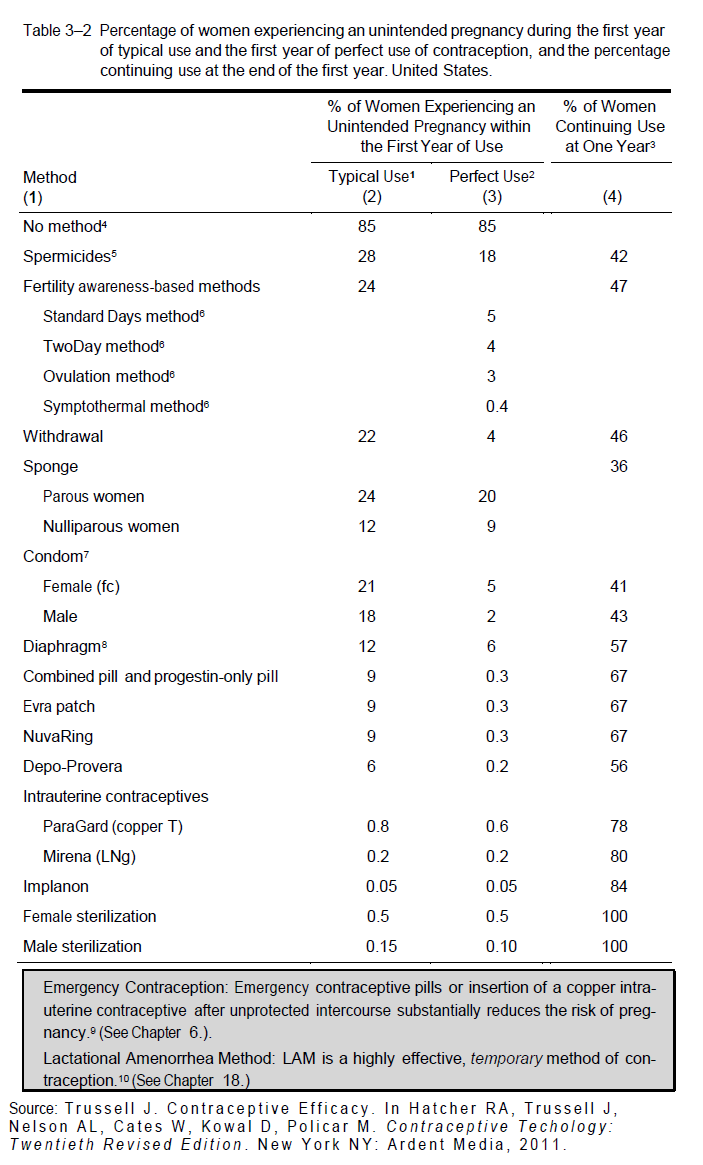
\includegraphics{"images/contraceptivefailure.png"}
\caption{\ldots{}}
\end{figure}
\end{column}
\end{columns}
\end{frame}

\begin{frame}{RCT Challenges: Spillovers! SUTVA}
\protect\hypertarget{rct-challenges-spillovers-sutva}{}
\begin{itemize}
\item
  Key RCT assumption: random assignment of D
\item
  Implicit RCT assumption:
  \textit{stable unit treatment value assumption} or \textit{SUTVA}.
\end{itemize}

\textbf{SUTVA: \textit{no spillovers.} Unit \(i\)'s potential outcomes
are unaffected by whether unit \(j\) is treated or untreated.}

SUTVA tends to be violated whenever the treatment, \(D_i\) involves
spillovers between groups, aka some type of externality.
\end{frame}

\begin{frame}{RCT Challenges: Spillovers! SUTVA}
\protect\hypertarget{rct-challenges-spillovers-sutva-1}{}
\begin{itemize}
\item
  Treatment: receiving a measles vaccination
\item
  Outcome: getting the measles
\end{itemize}

\textbf{Does SUTVA hold?}
\end{frame}

\begin{frame}{RCT Challenges: Spillovers! SUTVA}
\protect\hypertarget{rct-challenges-spillovers-sutva-2}{}
\begin{itemize}
\item
  Treatment: receiving a measles vaccination
\item
  Outcome: getting the measles
\end{itemize}

\textbf{Does SUTVA hold?}

\begin{itemize}
\item
  \(Y_i(D_i)\) depends on all of the \(D\)'s, not just \(D_i\).
\item
  Example: if all the units are vaccinated, except \(i\) then
  \(Y_i(1)-Y_i(0)=0\): no treatment effect. (Since there is no one for
  \(i\) to catch the measles from).
\end{itemize}

\textbf{What would be a potential SUTVA violation concern in our small
reading group simulation?}
\end{frame}

\begin{frame}{RCT Challenges: Attrition Bias}
\protect\hypertarget{rct-challenges-attrition-bias}{}
What happens to your estimates if some of the people in your experiment
vanish before you can collect their endline outcome data?

\begin{itemize}
\tightlist
\item
  If attrition is completely random, then it is not really a problem.
  Your sample size will be smaller but it will not bias your results.
\end{itemize}

But what will happen if attrition is a function of treatment status?

\begin{itemize}
\tightlist
\item
  RCT estimates are likely biased when attrition correlates with
  treatment status.
\end{itemize}
\end{frame}

\begin{frame}{Attrition Bias Simulation}
\protect\hypertarget{attrition-bias-simulation}{}
To see why, lets return to our simulation of the reading group RCT.

We know that the true treatment effect is \(\tau=10\).

Suppose there are missing scores: some students did not show up on test
day.

The students who do not show up are the students who know they will do
poorly on the reading exam.
\end{frame}

\begin{frame}[fragile]{Attrition Bias Simulation}
\protect\hypertarget{attrition-bias-simulation-1}{}
\tiny

\begin{Shaded}
\begin{Highlighting}[]
\NormalTok{scores5}\OperatorTok{$}\NormalTok{read4miss\textless{}{-}}\OtherTok{NA}
\NormalTok{scores5}\OperatorTok{$}\NormalTok{read4miss[scores5}\OperatorTok{$}\NormalTok{read4}\OperatorTok{\textgreater{}}\DecValTok{75}\NormalTok{]\textless{}{-}scores5}\OperatorTok{$}\NormalTok{read4[scores5}\OperatorTok{$}\NormalTok{read4}\OperatorTok{\textgreater{}}\DecValTok{75}\NormalTok{]}

\NormalTok{rctmiss\textless{}{-}}\KeywordTok{felm}\NormalTok{(read4miss}\OperatorTok{\textasciitilde{}}\NormalTok{treat,scores5)}

\KeywordTok{stargazer}\NormalTok{(rctmiss,  }\DataTypeTok{type=}\StringTok{"latex"}\NormalTok{, }\DataTypeTok{header=}\OtherTok{FALSE}\NormalTok{, }\DataTypeTok{omit.stat =} \StringTok{"all"}\NormalTok{)}
\end{Highlighting}
\end{Shaded}

\begin{table}[!htbp] \centering 
  \caption{} 
  \label{} 
\begin{tabular}{@{\extracolsep{5pt}}lc} 
\\[-1.8ex]\hline 
\hline \\[-1.8ex] 
 & \multicolumn{1}{c}{\textit{Dependent variable:}} \\ 
\cline{2-2} 
\\[-1.8ex] & read4miss \\ 
\hline \\[-1.8ex] 
 treat & 6.549$^{***}$ \\ 
  & (1.113) \\ 
  & \\ 
 Constant & 84.963$^{***}$ \\ 
  & (0.667) \\ 
  & \\ 
\hline \\[-1.8ex] 
\hline 
\hline \\[-1.8ex] 
\textit{Note:}  & \multicolumn{1}{r}{$^{*}$p$<$0.1; $^{**}$p$<$0.05; $^{***}$p$<$0.01} \\ 
\end{tabular} 
\end{table} 
\normalsize

Treatment:

\begin{itemize}
\item
  shifted the distribution upwards by 10 points
\item
  makes the ``observed'' left tale longer which biases our estimate
  downwards
\end{itemize}
\end{frame}

\begin{frame}{Addressing Attrition Bias}
\protect\hypertarget{addressing-attrition-bias}{}
Best option:

\begin{itemize}
\tightlist
\item
  Minimize attrition throughout the data collection process.
\end{itemize}

If you are still faced with attrition:

\begin{itemize}
\item
  check to see if there the attrition is similar across treatment and
  control groups
\item
  check if attrition correlates with observables
\end{itemize}

If you have uneven problematic attrition:

\begin{itemize}
\tightlist
\item
  it is sometimes possible to bound the extent of the bias by making
  hypothetical assumptions about who is dropping out of control and
  treatment.
\end{itemize}
\end{frame}

\begin{frame}{Attrition Bias Simulation}
\protect\hypertarget{attrition-bias-simulation-2}{}
If the principal knows that students who will score below 75 don't take
the test:

\begin{itemize}
\tightlist
\item
  she can recover the true treatment effect by excluding the students
  who became observed because of the treatment from the estimation
\end{itemize}

Of course it is unlikely that in the real world, a researcher would know
the exact model of attrition and how treatment affects attrition (ie the
treatment effect in this case).
\end{frame}

\begin{frame}[fragile]{Attrition Bias Simulation}
\protect\hypertarget{attrition-bias-simulation-3}{}
\tiny

\begin{Shaded}
\begin{Highlighting}[]
\NormalTok{scores5}\OperatorTok{$}\NormalTok{obsnew\textless{}{-}}\DecValTok{0}
\NormalTok{scores5}\OperatorTok{$}\NormalTok{obsnew[scores5}\OperatorTok{$}\NormalTok{treat}\OperatorTok{==}\DecValTok{1} \OperatorTok{\&}\StringTok{ }\NormalTok{scores5}\OperatorTok{$}\NormalTok{read4}\OperatorTok{\textgreater{}}\DecValTok{75} \OperatorTok{\&}\StringTok{ }\NormalTok{scores5}\OperatorTok{$}\NormalTok{read4}\OperatorTok{\textless{}}\DecValTok{85}\NormalTok{]\textless{}{-}}\DecValTok{1}

\NormalTok{rctmiss2\textless{}{-}}\KeywordTok{felm}\NormalTok{(read4miss}\OperatorTok{\textasciitilde{}}\NormalTok{treat,scores5[scores5}\OperatorTok{$}\NormalTok{obsnew}\OperatorTok{==}\DecValTok{0}\NormalTok{,])}


\KeywordTok{stargazer}\NormalTok{(rctmiss, rctmiss2, }\DataTypeTok{type=}\StringTok{"latex"}\NormalTok{, }\DataTypeTok{header=}\OtherTok{FALSE}\NormalTok{)}
\end{Highlighting}
\end{Shaded}

\begin{table}[!htbp] \centering 
  \caption{} 
  \label{} 
\begin{tabular}{@{\extracolsep{5pt}}lcc} 
\\[-1.8ex]\hline 
\hline \\[-1.8ex] 
 & \multicolumn{2}{c}{\textit{Dependent variable:}} \\ 
\cline{2-3} 
\\[-1.8ex] & \multicolumn{2}{c}{read4miss} \\ 
\\[-1.8ex] & (1) & (2)\\ 
\hline \\[-1.8ex] 
 treat & 6.549$^{***}$ & 10.240$^{***}$ \\ 
  & (1.113) & (1.102) \\ 
  & & \\ 
 Constant & 84.963$^{***}$ & 84.963$^{***}$ \\ 
  & (0.667) & (0.597) \\ 
  & & \\ 
\hline \\[-1.8ex] 
Observations & 195 & 177 \\ 
R$^{2}$ & 0.152 & 0.330 \\ 
Adjusted R$^{2}$ & 0.148 & 0.327 \\ 
Residual Std. Error & 7.455 (df = 193) & 6.677 (df = 175) \\ 
\hline 
\hline \\[-1.8ex] 
\textit{Note:}  & \multicolumn{2}{r}{$^{*}$p$<$0.1; $^{**}$p$<$0.05; $^{***}$p$<$0.01} \\ 
\end{tabular} 
\end{table}
\end{frame}

\begin{frame}{RCT advantages:}
\protect\hypertarget{rct-advantages}{}
\begin{itemize}
\item
  Randomized Control trials: huge advantages for causal inference.
\item
  RCTs are relatively easy to explain to policy makers, and even the
  general public \(\Rightarrow\) important advantages when it comes to
  communicating research results to the wider world.
\item
  RCT have become a widely used tool in economics and the social
  sciences today.
\item
  The 2019 Nobel Laureat in Economics was give to Abhijit Banerjee,
  Esther Duflo and Michael Kremer for their role in bringing this
  experimental approach to economic research (particularly in
  development economics).
\end{itemize}
\end{frame}

\begin{frame}{RCT limitations:}
\protect\hypertarget{rct-limitations}{}
RCT's can be quite costly to conduct and the logistics of running an RCT
are quite demanding.

Many very important social and economic questions where running an RCT
would simply not be ethical.

\begin{itemize}
\tightlist
\item
  the effects of juvenile incarceration on human capital and future
  crime is clearly a question of first order importance but
  randomization would clearly be unethical.
\end{itemize}

Conceptual limitations:

\begin{itemize}
\item
  External validity
\item
  Experimenter demand effects
\item
  General equilibrium effects
\end{itemize}
\end{frame}

\begin{frame}{External validity}
\protect\hypertarget{external-validity}{}
Would you get the same results in a different context?

\begin{itemize}
\tightlist
\item
  RCT's are often conducted in a limited geographical area with a
  relatively small sample size.
\end{itemize}

Would you get the same results if the program were implemented on a
larger scale?

\begin{itemize}
\tightlist
\item
  RCT's are often implemented with a lot more care and resources more
  then the large scale policy they are testing. This could change the
  effects.
\end{itemize}
\end{frame}

\begin{frame}{Experimenter demand effects}
\protect\hypertarget{experimenter-demand-effects}{}
Could subjects be behaving differently then they normally would because
of the experimental context they are in?

\begin{itemize}
\item
  \textbf{Hawthorne effects:} the idea that individuals might modify
  their behavior simply because they are being observed.
\item
  a particular concern, if they would affect the treatment and control
  differently.
\end{itemize}

Are subjects changeing their behavior in order to conform to what they
believe the researcher expects of them?

\begin{itemize}
\tightlist
\item
  This is a particularly important question when experiments are
  incentivized and a subject could perceive that they would receive more
  rewards for certain types of behaviors.
\end{itemize}
\end{frame}

\begin{frame}{Experimenter demand effects}
\protect\hypertarget{experimenter-demand-effects-1}{}
Generally advisable to:

\begin{itemize}
\item
  Minimize the salience of the evaluation
\item
  Ensure the experimental experience is the same for both the treated
  and control groups.
\end{itemize}
\end{frame}

\begin{frame}{General equilibrium effects}
\protect\hypertarget{general-equilibrium-effects}{}
Many of the policies we are interested in in economics affect variables
that are not determined by a single individual's choices (eg prices).

Most RCT's are small: unlikely to affect market level variables such as
prices.

If the intervention were implemented at scale, could changes in market
level variables change estimated effects?
\end{frame}

\begin{frame}{Fishing for Stars}
\protect\hypertarget{fishing-for-stars}{}
Other research issues (not exclusive to RCT's):

\begin{itemize}
\item
  Publication Bias
\item
  P-Hacking
\item
  Cherry-Picking
\item
  The push for research transparency
\end{itemize}

Note: these points are most relevant for academic research, but
highlight the need to understand the incentives behind any data analysis
project.
\end{frame}

\begin{frame}{Publication Bias}
\protect\hypertarget{publication-bias}{}
\begin{itemize}
\item
  Common problem in many scientific fields.
\item
  Papers that report null-results (ie, no statistically significant
  effect was detected) are much more difficult to publish
\item
  These papers may be left unwritten leading to the ``file drawer''
  problem:

  \begin{itemize}
  \item
    null-results are unobserved \(\Rightarrow\) an incomplete picture to
    the answer to important questions
  \item
    wasted effort as researchers re-do analysis that has already been
    done but was never publicized.
  \end{itemize}
\end{itemize}
\end{frame}

\begin{frame}{Publication Bias}
\protect\hypertarget{publication-bias-1}{}
\centering \includegraphics[width=0.65\textwidth,height=\textheight]{"images/mervis.png"}
\end{frame}

\begin{frame}{P-Hacking}
\protect\hypertarget{p-hacking}{}
When choosing between different (valid) ways to specify a regression,
researchers will often favor the most ``publishable'' results.

\centering 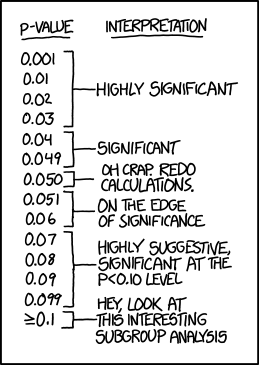
\includegraphics[width=0.4\textwidth,height=\textheight]{"images/phackingcomic.png"}
\end{frame}

\begin{frame}{P-Hacking}
\protect\hypertarget{p-hacking-1}{}
This leads to an excess mass of papers reporting p-values that are right
under the ``significance'' (z=1.96) threshold.

\begin{figure}
\centering
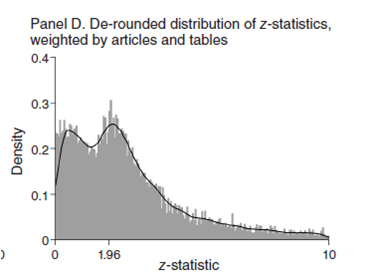
\includegraphics[width=0.65\textwidth,height=\textheight]{"images/brodeuretal.png"}
\caption{From Brodeur et al.2016}
\end{figure}
\end{frame}

\begin{frame}{P-Hacking}
\protect\hypertarget{p-hacking-2}{}
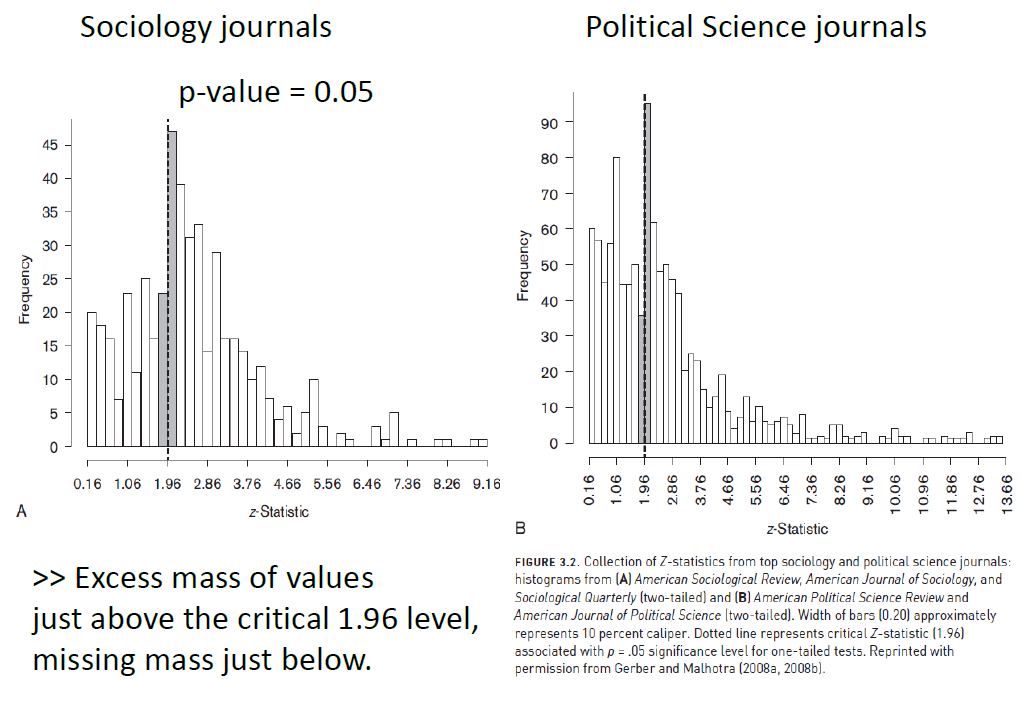
\includegraphics[width=0.85\textwidth,height=\textheight]{"images/pvalpolsci.png"}
\end{frame}

\begin{frame}{Cherry-Picking}
\protect\hypertarget{cherry-picking}{}
\includegraphics{"images/significant_comic1.png"}
\end{frame}

\begin{frame}{Cherry-Picking}
\protect\hypertarget{cherry-picking-1}{}
\includegraphics{"images/significant_comic2.png"}
\end{frame}

\begin{frame}{Cherry-Picking}
\protect\hypertarget{cherry-picking-2}{}
\includegraphics{"images/significant_comic3.png"}
\end{frame}

\begin{frame}{Cherry-Picking}
\protect\hypertarget{cherry-picking-3}{}
\includegraphics{"images/significant_comic4.png"}
\end{frame}

\begin{frame}{Cherry-Picking}
\protect\hypertarget{cherry-picking-4}{}
When researchers have incurred large costs on a project, there are very
strong incentives to find significant effects.

One way to increase the chance of finding significant effects, is to
collect data on a huge number of outcome variables.

Without insight into the actual research process, it then becomes
difficult to tell if the researcher found what their hypothesis
predicted or if they simply ran many many regressions.
\end{frame}

\begin{frame}{Efforts towards research transparency}
\protect\hypertarget{efforts-towards-research-transparency}{}
There is a push to address these issues in economics, particularly in
the RCT field.

\begin{itemize}
\item
  \textbf{Public Data and Code:} Increasingly a journal requirement
\item
  \textbf{Multiple inference adjusted standard errors:} report adjusted
  standard errors to compensate for the number of inferences being made,
  if there are many outcomes.
\item
  \textbf{Pre-analysis plans:} a publicly filed document detailing the
  the questions, methods, and estimations a researcher plans to
  implement before they actually receive any data.
\item
  \textbf{Pre-result publication:} Some journals are starting to accept
  articles based on the pre-analysis plan, before seeing any results.
\end{itemize}
\end{frame}

\begin{frame}{Efforts towards research transparency}
\protect\hypertarget{efforts-towards-research-transparency-1}{}
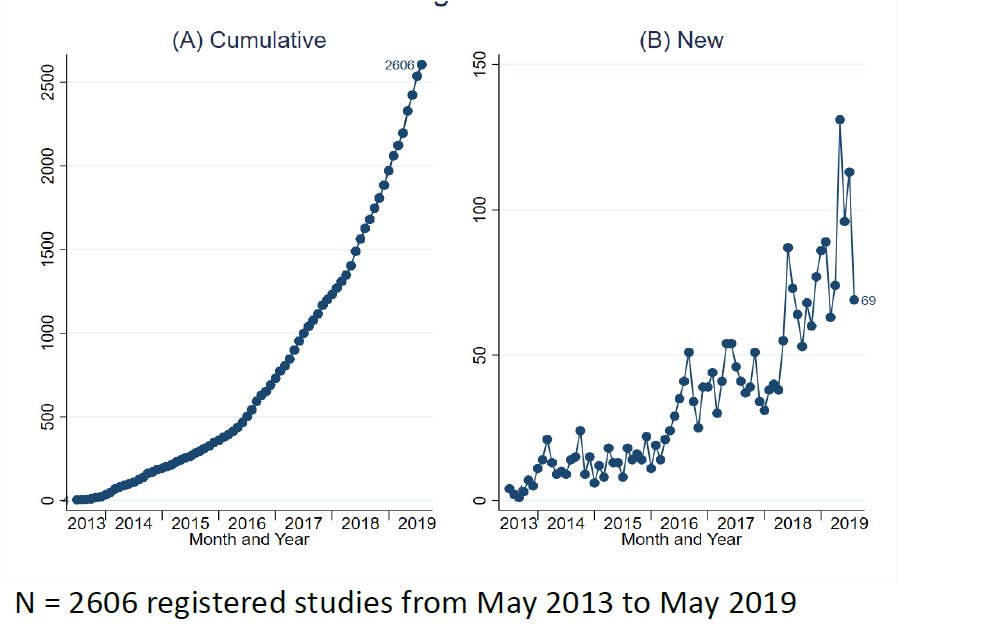
\includegraphics{"images/PAP.png"}
\end{frame}

\end{document}
